\section{Технический проект}

\subsection{Общая характеристика организации решения задачи}
Обсуждение методологии разработки, включая Agile подходы, планирование спринтов и процессы контроля качества, основывается на принципах эффективной работы в условиях быстро меняющихся требований, как описано в источнике~\cite{yordon}.

\subsection{Обоснование выбора технологий проектирования}
\subsubsection{.NET Core}
Выбор .NET Core для серверной разработки обосновывается его производительностью, масштабируемостью и кросс-платформенностью, а также поддержкой работы с админ-панелью <<из коробки>>, что является важным фактором в современной разработке программного обеспечения, как отмечено в~\cite{mark_price}.
Начиная с версии .NET core 6.0, которая была выбрана для разработки, поддерживается работа с админ-панелью <<из коробки>>, что позволяет сэкономить ресурсы на разработки панели администратора.

\subsubsection{Entity Framework Core}
Entity Framework Core является ORM (Object-Relational Mapping) для .NET Core. Он позволяет работать с базами данных, используя объектно-ориентированный подход~\cite{grinchenko}. Entity Framework Core позволяет работать с различными СУБД, в том числе с PostgreSQL, которая была выбрана для разработки.

\subsubsection{PostgreSQL}
Выбор PostgreSQL в качестве системы управления базами данных был обусловлен её высокой надежностью, поддержкой продвинутых SQL-функций и совместимостью с Entity Framework Core. PostgreSQL предлагает удобные функции для разработчиков, такие как JSON/JSONB поддержка, хранение процедур и триггеры, что делает её идеальной для комплексных приложений, требующих масштабируемости и гибкости. К тому же, PostgreSQL обладает мощными средствами для работы с большими объемами данных и комплексными запросами, что критично для обеспечения высокой производительности приложения.

\subsubsection{Angular}
Angular, выбранный для Frontend разработки, предоставляет строгую и требовательную архитектуру, что делает его идеальным инструментом для создания сложных и масштабируемых приложений. Эффективность Angular в разработке интерактивных интерфейсов и легкость интеграции с REST API подчеркивается в~\cite{cssspecs}.

\subsection{Проектирование пользовательского интерфейса}

На основании требований к пользовательскому интерфейсу, представленных в пункте 2.3 технического задания, был разработан графический интерфейс мобильного приложения, используя Angular с применением HTML, JavaScript и SCSS. Этот процесс подчеркивает важность интуитивно понятного и эффективного взаимодействия с пользователем, как отмечено в~\cite{kumskova}.
Разработанный интерфейс ориентирован на обеспечение легкости в использовании и интуитивного понимания функционала приложения, предоставляя пользователю гладкое и эффективное взаимодействие с приложением.

\begin{enumerate}
    \item \textbf{Поиск}: Реализация функции поиска на основе поля \textit{ProductName} из класса \textit{Product}, \textit{Price}, \textit{Weight}, и \textit{ProductGroupId} класса \textit{Product}.
    \item \textbf{Отображение результатов поиска}: Эффективное представление списка товаров, включая \textit{ImageUrl}, \textit{ProductName}, информацию о \textit{Category} и \textit{Price}.
    \item \textbf{Детали товара}: Дополнительная информация о товаре, включая его \textit{Category} и \textit{Weight}.
    \item \textbf{Навигация по приложению}: Элементы навигации, такие как кнопка возврата к началу списка и индикаторы категорий.
\end{enumerate}

\begin{figure}[h!]
    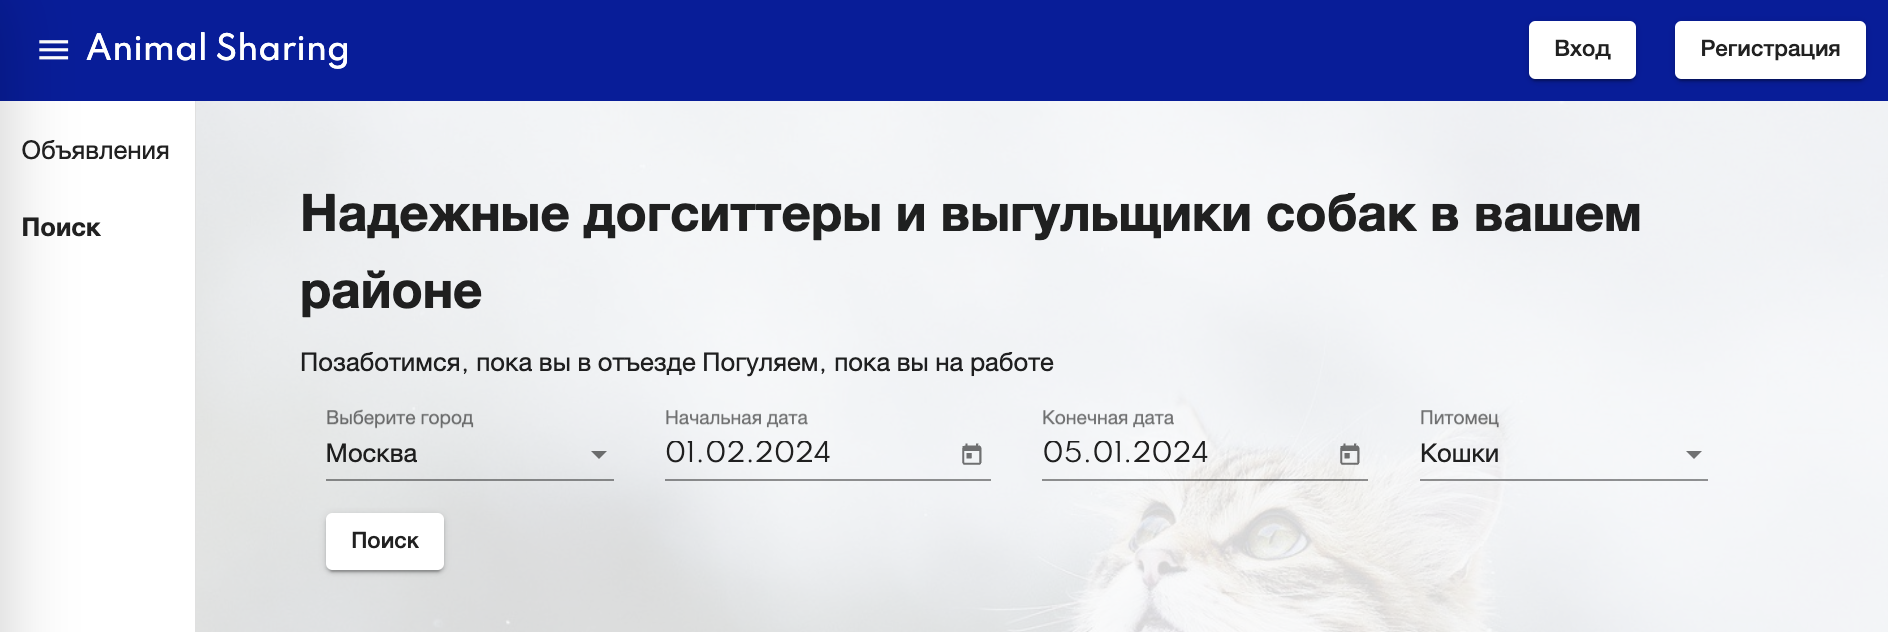
\includegraphics[width=0.82\linewidth]{interface-search.png}
    \caption{модели интерфейса <<Поиск>> и <<Навигация по приложению>>}
    \label{fig:search}
\end{figure}

Процесс регистрации пользователя в приложении максимально упрощен и включает следующие шаги:
\begin{enumerate}
    \item Пользователь выбирает опцию <<Регистрация>> на главном экране.
    \item Заполняются основные поля: электронная почта, имя пользователя и пароль.
    \item Пользователь должен подтвердить свой адрес электронной почты через полученное письмо со ссылкой для подтверждения.
    \item После подтверждения электронной почты, пользователь может ввести дополнительную информацию в свой профиль: фотографию, контактные данные и предпочтения в приложении.
    \item На последнем этапе пользователь принимает условия пользования и политику конфиденциальности, после чего регистрация завершается.
\end{enumerate}

Регистрация дог-ситтеров предполагает прохождение дополнительных этапов для верификации и предоставления информации о предоставляемых услугах:
\begin{enumerate}
    \item Потенциальный дог-ситтер начинает регистрацию с выбора соответствующего пункта в приложении.
    \item Вводятся личные данные, включая полное имя, адрес проживания и номер телефона.
    \item Запрашивается информация о предыдущем опыте работы с животными и наличии соответствующих рекомендаций.
    \item Дог-ситтер должен пройти онлайн-курс по уходу за животными и предоставить сертификат о его окончании.
    \item Предоставляется информация об услугах, включая доступные даты и временные рамки, а также устанавливаются тарифы.
    \item Профиль дог-ситтера отправляется на проверку. После одобрения администрацией профиль становится доступным для поиска и выбора пользователями.
\end{enumerate}


\begin{figure}[h!]
    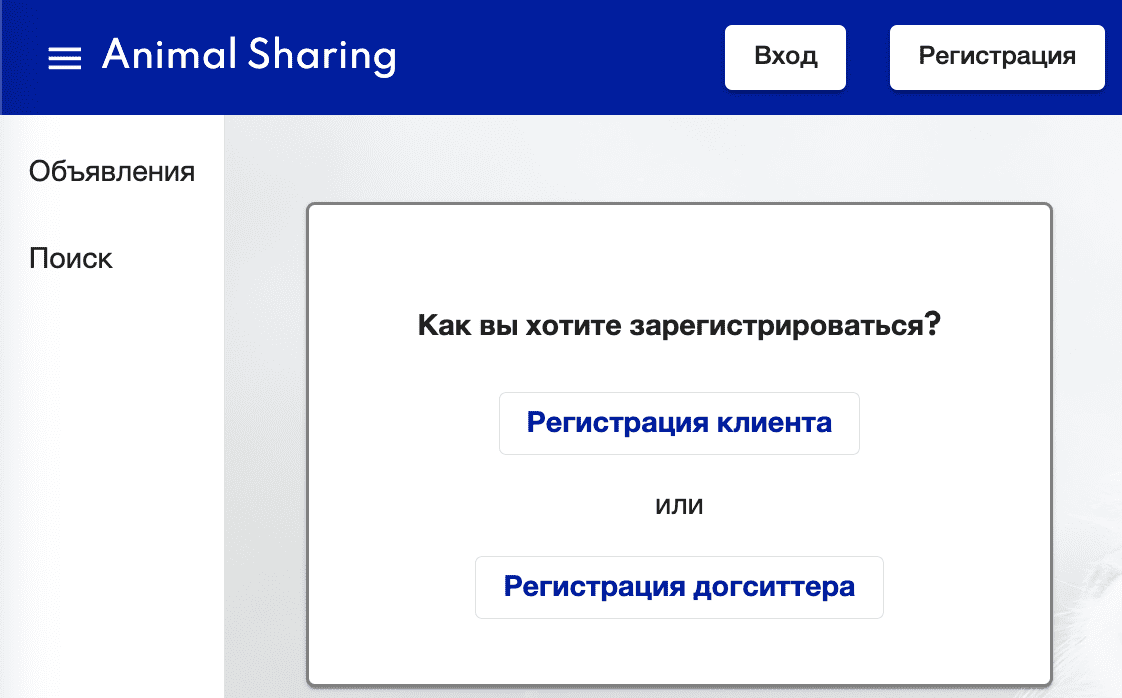
\includegraphics[width=0.82\linewidth]{interface-register.png}
    \caption{Модели интерфейса регистрации <<Пользователя>> и <<Дог-ситтера>>}
    \label{fig:register}
\end{figure}

\subsection{Диаграмма размещения}
Диаграмма размещения (рис.~\ref{place:image}) иллюстрирует физические взаимосвязи между программными и аппаратными компонентами системы, подчеркивая важность стратегического планирования в разработке распределенных систем, как отмечено в~\cite{makni}.

\begin{figure}[ht]
\center{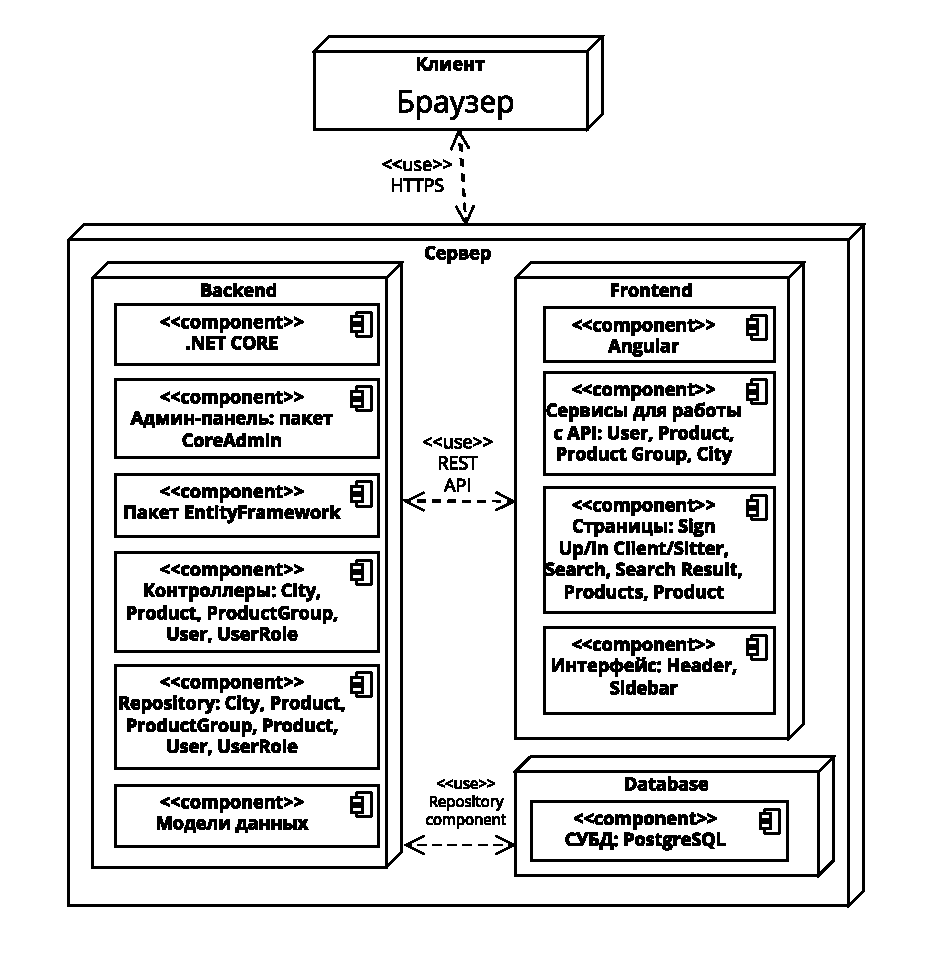
\includegraphics[width=1\linewidth]{client-server.eps}}
\caption{Диаграмма размещения}
\label{place:image}
\end{figure}

Она является хорошим средством для показа маршрутов перемещения объектов и компонентов в распределенной системе.

\subsection{Описание классов системы}

\subsubsection{Описание классов серверной части}

\begin{itemize}
    \item <<UserBase>> служит основой для всех пользовательских данных, предоставляя общие поля, такие как <<Phone>>, <<Email>>, <<FirstName>>, <<LastName>>, и т.д.
    \item <<UserRegistrationData>> расширяет <<UserBase>>, добавляя специфичное для регистрации поле <<Password>>.
    \item <<UserLoginData>> используется для процесса входа в систему, содержа только <<Email>> и <<Password>>.
    \item <<UserLoginResponseData>> и <<UserView>> расширяют <<UserBase>>, добавляя уникальный идентификатор <<Id>>, а <<UserLoginResponseData>> также включает <<AccessToken>> для аутентификации.
    \item <<User>> является полным представлением пользователя, включающим безопасность (через <<Hash>> и <<Salt>>) и <<Id>>.
\end{itemize}

% Таблица для UserBase
\begin{xltabular}{\textwidth}{|l|l|p{1.7cm}|X|}
    \caption{Атрибуты сущности <<UserBase>>}\\ \hline
    Поле & Тип & Обяза\-тельное & Описание \\ \hline
    Phone & String & false & Телефонный номер пользователя \\ \hline
    Email & String & false & Электронная почта пользователя \\ \hline
    FirstName & String & false & Имя пользователя \\ \hline
    LastName & String & false & Фамилия пользователя \\ \hline
    ImageUrl & String & false & URL изображения пользователя \\ \hline
    Telegram & String & false & Telegram пользователя \\ \hline
    Website & String & false & Веб-сайт пользователя \\ \hline
\end{xltabular}

% Таблица для UserRegistrationData
\begin{xltabular}{\textwidth}{|l|l|p{1.7cm}|X|}
    \caption{Атрибуты сущности <<UserRegistrationData>>}\\ \hline
    Поле & Тип & Обяза\-тельное & Описание \\ \hline
    % Здесь перечислены атрибуты из UserBase
    Password & String & true & Пароль пользователя \\ \hline
\end{xltabular}

% Таблица для UserLoginData
\begin{xltabular}{\textwidth}{|l|l|p{1.7cm}|X|}
    \caption{Атрибуты сущности <<UserLoginData>>}\\ \hline
    Поле & Тип & Обяза\-тельное & Описание \\ \hline
    Email & String & true & Электронная почта пользователя для входа \\ \hline
    Password & String & true & Пароль пользователя для входа \\ \hline
\end{xltabular}

% Таблица для UserLoginResponseData
\begin{xltabular}{\textwidth}{|l|l|p{1.7cm}|X|}
    \caption{Атрибуты сущности <<UserLoginResponseData>>}\\ \hline
    Поле & Тип & Обяза\-тельное & Описание \\ \hline
    % Здесь перечислены атрибуты из UserBase
    Id & Long & true & Уникальный идентификатор пользователя \\ \hline
    AccessToken & String & true & Токен доступа пользователя \\ \hline
\end{xltabular}

% Таблица для UserView
\begin{xltabular}{\textwidth}{|l|l|p{1.7cm}|X|}
    \caption{Атрибуты сущности <<UserView>>}\\ \hline
    Поле & Тип & Обяза\-тельное & Описание \\ \hline
    % Здесь перечислены атрибуты из UserBase
    Id & Long & true & Уникальный идентификатор пользователя \\ \hline
\end{xltabular}

% Таблица для User
\begin{xltabular}{\textwidth}{|l|l|p{1.7cm}|X|}
    \caption{Атрибуты сущности <<User>>}\\ \hline
    Поле & Тип & Обяза\-тельное & Описание \\ \hline
    % Здесь перечислены атрибуты из UserBase
    Id & Long & true & Уникальный идентификатор пользователя \\ \hline
    Hash & String & true & Хэш пользователя \\ \hline
    Salt & String & true & Соль для хэша пароля пользователя \\ \hline
\end{xltabular}

\begin{itemize}
    \item <<Product>>, наследующийся от <<Short>>, описывает основную информацию о продукте, такую как <<ImageUrl>>, <<ProductGroupId>>, <<Price>>, <<Weight>>, и <<CreatedByUserId>>, указывающий на пользователя, создавшего продукт.
    \item <<ProductView>> расширяет <<Product>>, добавляя <<CreatedByUser>>, который является экземпляром <<UserView>>. Это позволяет получать не только идентификационную информацию о создателе продукта, но и более детальные данные пользователя.
\end{itemize}

% Таблица для Product
\begin{xltabular}{\textwidth}{|l|l|p{1.7cm}|X|}
    \caption{Атрибуты сущности <<Product>>}\\ \hline
    Поле & Тип & Обяза\-тельное & Описание \\ \hline
    % Здесь перечислены атрибуты из Short
    ImageUrl & String & false & URL изображения продукта \\ \hline
    ProductGroupId & Long & true & Идентификатор группы продуктов \\ \hline
    Price & Float & true & Цена продукта \\ \hline
    Weight & Integer & true & Вес продукта \\ \hline
    CreatedByUserId & Long & true & Идентификатор пользователя, создавшего продукт \\ \hline
\end{xltabular}

% Таблица для ProductView
\begin{xltabular}{\textwidth}{|l|l|p{1.7cm}|X|}
    \caption{Атрибуты сущности <<ProductView>>}\\ \hline
    Поле & Тип & Обяза\-тельное & Описание \\ \hline
    % Здесь перечислены атрибуты из Product
    CreatedByUser & UserView & true & Пользователь, создавший продукт \\ \hline
\end{xltabular}

Описание классов серверной части включает <<UserBase>>, <<UserRegistrationData>>, <<UserLoginData>>, <<UserLoginResponseData>> и <<User>>, отражая разнообразие и сложность структур данных в современных системах. Подход к проектированию и реализации этих классов основывается на объектно-ориентированных принципах и практиках, отмеченных в~\cite{grinchenko} и~\cite{kumskova}.

В системе предусмотрен внутренний механизм связи между разделами и элементами информационных блоков, поэтому введения дополнительных идентификаторов при реализации связей между сущностями не предполагается.

Экземпляры сущностей реализуются в информационных блоках посредством элементов, атрибуты сущности – посредством полей и свойств элемента.

\subsubsection{Описание классов клиентской части}

\begin{itemize}
    \item <<Short>> -\- основной интерфейс, используемый для предоставления общей структуры данных. Поля <<id>>, <<name>> и <<description>> являются фундаментальными для большинства сущностей;
    \item <<User>> -\- расширяет <<Short>>, интегрируя контактные данные и личную информацию пользователя. Используется для управления учетными записями пользователей, включая процессы регистрации и авторизации;
    \item <<ProductGroup>> -\- расширяет <<Short>>, добавляя конкретные детали для организации продуктов в группы. Используется для классификации и управления ассортиментом продуктов;
    \item <<Product>> -\- расширяет <<Short>>, предоставляя подробную информацию о продуктах. Включает данные о создателе продукта и используется для представления конкретных товаров в системе;
    \item <<City>> -\- описывает города, с полями <<id>> и <<name>>. Используется для управления информацией о местоположениях, связанных с пользователями и продуктами.
\end{itemize}

% Таблица для Short
\begin{xltabular}{\textwidth}{|l|l|p{1.7cm}|X|}
    \caption{Атрибуты интерфейса <<Short>>}\\ \hline
    Поле & Тип & Обяза\-тельное & Описание \\ \hline
    id & number & true & Уникальный идентификатор \\ \hline
    name & string & true & Название \\ \hline
    description & string & true & Описание \\ \hline
\end{xltabular}

% Таблица для User
\begin{xltabular}{\textwidth}{|l|l|p{1.7cm}|X|}
    \caption{Атрибуты интерфейса <<User>>}\\ \hline
    % Здесь перечислены атрибуты из Short
    phone & string & false & Телефонный номер \\ \hline
    % ... другие поля User ...
    accessToken & string & false & Токен доступа \\ \hline
\end{xltabular}

% Таблица для ProductGroup
\begin{xltabular}{\textwidth}{|l|l|p{1.7cm}|X|}
    \caption{Атрибуты интерфейса <<ProductGroup>>}\\ \hline
    % Здесь перечислены атрибуты из Short
    type & string & true & Тип группы продуктов \\ \hline
    % ... другие поля ProductGroup ...
\end{xltabular}

% Таблица для Product
\begin{xltabular}{\textwidth}{|l|l|p{1.7cm}|X|}
    \caption{Атрибуты интерфейса <<Product>>}\\ \hline
    % Здесь перечислены атрибуты из Short
    imageUrl & string & false & URL изображения продукта \\ \hline
    % ... другие поля Product ...
\end{xltabular}

% Таблица для City
\begin{xltabular}{\textwidth}{|l|l|p{1.7cm}|X|}
    \caption{Атрибуты интерфейса <<City>>}\\ \hline
    id & number & true & Уникальный идентификатор \\ \hline
    name & string & true & Название города \\ \hline
\end{xltabular}

